\documentclass[bwprint]{gmcmthesis}
\usepackage{amsmath}
\numberwithin{figure}{section}
\renewcommand{\thefigure}{\arabic{section}-\arabic{figure}}
\usepackage{tabularx}
\usepackage{array}
\usepackage{makecell}
\usepackage{tabu}
\usepackage{longtable}
\usepackage{booktabs}
\usepackage{amsmath}
\usepackage{pdflscape}
\usepackage{cite}




\newcolumntype{Y}{>{\centering\arraybackslash}X}
% \documentclass[withoutpreface,bwprint]{cumcmthesis}
% 去掉封面与编号页

\title{机场新增卫星厅对中转旅客影响的研究}
\baominghao{No.00000001} %参赛队号
\schoolname{东南大学}%学校名称
\membera{张昀蔚} %队员A
\memberb{刘梦阳} %队员B
\memberc{王喻星} %队员C
\begin{document}
 \maketitle
 \begin{abstract}
本文以最优化原理为理论基础,对航班-登机口的优化分配问题进行研究,并在此基础上评价终端厅对中转旅客的影响程度。针对三个问题,本模型在考虑航班分配失败率最小、被使用登机口比率最小的同时分别以最小化中转旅客总体最短流程时间和总体紧张度为研究目标,建立多目标多约束的登机口分配优化模型,利用生物地理学算法进行步步寻优,但研究中也发现,在最小化中转旅客总体最短流程时间和总体紧张度的过程中,导致分配到临时登机口的旅客人数较多,尤其是旅客人数较多的航班会倾向于分配到临时机位;针对这个现象,本文采用惩罚机制来限制分配到临时机位的航班数量,对比验证了惩罚机制对于航班分配的影响。

\textbf{问题一}:在不考虑中转旅客换乘问题的基础上,建立以航班分配失败率最小和被使用登机口比率最小为目标的双目标多约束优化模型,结合登机口分配规则、飞机指派规则、机体型号等约束条件,利用生物地理学算法对该模型进行求解。结果表明:成功分配登机口的航班比例为 82.18\%,被使用登机口数量为 65 个。

\textbf{问题二}:在问题一的基础上,考虑中转旅客的总体最短流程时间,按照以航班分配失败率最小(目标一)、中转旅客总体最短流程时间最小(目标二)以及被使用登机口比率最小(目标三)为优先级,建立多目标多约束的登机口分配优化模型。利用生物地理学算法通过不断的收敛逐渐得到最优解。结果发现,成功分配登机口的航班比例为 77.56\%,中转旅客总体最短流程时间为 50350 分钟,被使用登机口数量为 64 个。由于分配到临时登机口的旅客最短流程时间并不计入总体最短流程时间,我们发现在进行目标函数一和二的优化过程中,承载旅客数量较少的航班更容易分配到固定登机口,而承载旅客数量较多的航班倾向于分配到临时登机口,通过计算以上结果,发现共有 1197 人分配到临时登机口,同样会损害航空公司的利益。所以针对问题二本文提出第二种目标函数,即将分配到临时登机口的旅客加入惩罚时间 6 小时计入总最短流程时间,结果发现虽然被使用登机口数量增加为 67 个,总换乘时间增加至 69480 分钟,但是只有 699 个乘客分配至临时登机口。

\textbf{问题三}:在问题二的基础上,考虑中转旅客的换乘时间,按照以航班分配失败率最小(目标一)、中转旅客总体紧张度最小(目标二)以及被使用登机口比率最小(目标三)为优先级,建立多目标多约束的登机口分配优化模型。利用生物地理学算法通过不断的收敛逐渐得到最优解。同样,当临时登机口旅客得惩罚时间不计入换乘时间,即不影响旅客总体紧张度的情况下,成功分配登机口的航班比例为 79.21\%,旅客总体紧张度为 454.33,被使用登机口数量为 66 个,而1193个旅客被分配至临时登机口;当临时登机口旅客的惩罚时间计入换乘时间,成功分配登机口的航班比例增加为 82.84\%,旅客总体紧张度增加为 607.26,被使用登机口数量保持 66 个,但是只有 726 个乘客分配至临时登机口。

综上所述,本文提出的多目标多约束的登机口分配优化模型能恰当地描述不同目标以及约束条件下航班-登机口地分配问题,而且采用生物地理学算法可快速求解该模型,二者的组合是一种行之有效的登机口分配方案。


\keywords{登机口分配, 多目标多约束,  航班分配失败率,  最短流程时间,  总体紧张度,  被使用登机口比率,  生物地理学算法}
\end{abstract}

%\pagestyle{plain}

%目录
\tableofcontents

\newpage
\section{问题重述}
\subsection{研究背景}
随着我国航空运输的快速发展,急剧增长的客货运输量对民航运输需求不断增加。现有的航站楼旅客的客流量已经达到饱和状态,为了应对不断增加的客流量对机场带来的巨大压力,某机场正在增设卫星厅;虽然卫星厅可以很大程度上的缓解原有航站楼登机口不足的问题,但是对于部分中转旅客而言,会增加其在转场过程中所需要的换乘时间,进而加剧中转旅客的换乘紧张程度,使得旅客对于航空公司和机场的服务满意度降低。

机场资源的有限性是限制枢纽机场发展的重要因素之一,如何提高中转旅客效率已经成为改善枢纽机场中转运行效率的关键性问题,也是其实现自身枢纽战略目标的关键性技术\cite{bouras2014airport, marinelli2015metaheuristic}。在进行航班换乘时,航班和登机口的衔接指派上也面临着资源的合理调度问题,需要通过技术手段对登机口进行合理指派从而保证有限的登机口资源实现利用最大化,同时考虑旅客的换乘体验\cite{zhang2017multi}。对于单纯的航班—登机口优化分配问题已经被很好的解决,而且有非常成熟的产品满足航空公司和机场地勤服务公司的需求。但是如何在优化分配登机口的同时考虑旅客换乘时间最小,这方面的研究还是相对较少。登机口优化分配有两个关键因素需要考虑:一是创建合适的数学优化模型;二是找到合适的算法快速求解该数学模型。在实际应用过程中,创建更加符合实际需求的数学模型和采用行之有效的求解算法是解决优化分配问题的关键。
\subsection{已知信息}
\begin{enumerate}[label={(\arabic*)}]
\item 
已知机场的航站楼 T 和航站楼 S 的布局设计、两航站楼登机口的功能属性、不同航站楼登机口间的换乘时间、登机口分配规则、旅客流程等;
\item
已知 2018 年 1 月 19、20、21 号三天的出发、到达航班的旅客数据、航班信息。
\end{enumerate}
\subsection{需要解决的问题}
基于已知信息建立数学模型,并在给定的航班数据、旅客信息下,求解以下三个问题:

问题一:航班-登机口分配问题。作为分析新建卫星厅对航班影响问题的第一步,首先要建立登机口优化分配数学模型,不考虑中转旅客的换乘问题,尽可能多地分配航班到合适的登机口,并且在此基础上最小化被使用登机口的数量。

问题二:考虑中转旅客最短流程时间的航班-登机口分配问题。本问题是在问题一的基础上加入旅客换乘因素,考虑中转旅客的到达航班和出发航班的飞机所在的登机口的位置对旅客中转流程时间的影响,要求在登机口分配过程中首先考虑航班分配成功数量最大及中转旅客的总体最短流程时间最短,并且在此基础上进一步最小化被使用登机口的数量,进而得到一个多目标优化模型。本问题不考虑换乘旅客乘坐捷运和步行时间。

问题三:考虑中转旅客的换乘时间的航班-登机口分配问题。在登机口分配过程中,新建卫星厅对航班存在的最大影响是中转旅客的换乘时间可能会增加,进而导致部分中转旅客无法及时换乘后续航班;本问题中将换乘旅客的最短流程时间、捷运时间以及步行时间之和作为旅客的换乘时间,旅客的换乘时间转换为旅客换乘紧张度,在进行航班-登机口分配的过程中,首先优化航班分配成功数量最大及中转旅客的总体换乘紧张度最小,并且在此基础上进一步最小化被使用登机口的数量,进而得到一个多目标优化模型。

\section{模型假设}
\begin{enumerate}[label={(\arabic*)}]
\item 假设题目中涉及的航班时间均为国际标准时间。
\item 假设题目中涉及的旅客均为换乘旅客,不考虑始发旅客和终到旅客。
\item 假设航班的实际到达时间、实际出发时间与航班计划一致,不受天气状况、管制等其他因素干扰。
\item 设置临时机位,且临时机位的数量不受限制,保证每架飞机均能指派到一个登机口。
\item 研究时段内的所有航班信息和旅客中转信息是已知的。
\item 假设旅客中转过程中的换乘时间与登机口位置有关,是相对固定的,不考虑人为随机因素的影响。
\item 登机口指派是一个连续过程,本文选择一段时间内的飞机进行指派。
\end{enumerate}


%\begin{figure}[!h]
%\centering
%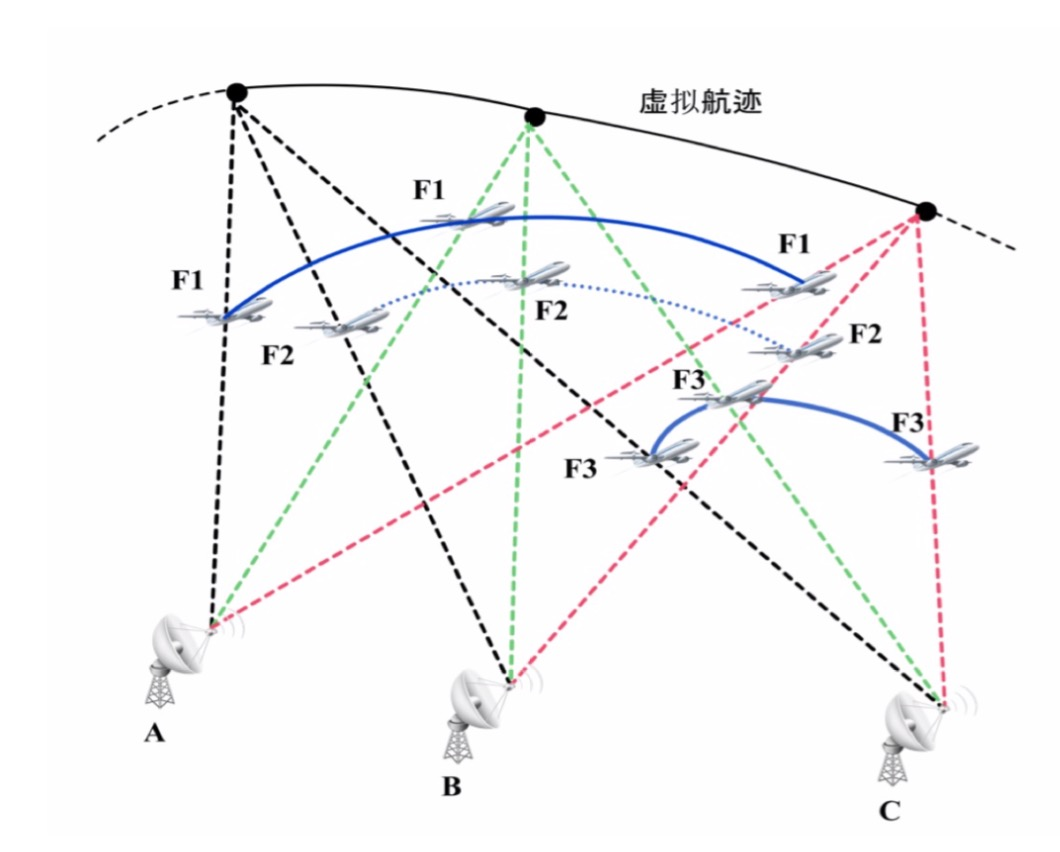
\includegraphics[width=.7\textwidth]{test.jpg}
%\caption{对雷达实施距离多假目标欺骗干扰示意图}
%\label{fig1}
%\end{figure}

\section{符号说明}
\renewcommand	\arraystretch{1.5} %设置行距
\begin{longtable}{m{4cm}<{\centering} m{\textwidth-4cm}<{\centering}}	
\caption{符号说明} \label{tab:symbol} \\ 
\Xcline{1-2}{2pt}
\endfirsthead
\Xcline{1-2}{2pt}
\endlastfoot
\caption{(续)}\\
\Xcline{1-2}{2pt}
符号                 & 变量说明   \\
\hline
\endhead
\Xcline{1-2}{2pt}
\endfoot
符号                 & 变量说明   \\
\hline
$F$                   & 飞机集合   \\  
$f_i$                & 飞机编号    \\  
$C_{f_i}$       & 飞机型号    \\  
$C_{f_i}^a$   & 飞机到达类型 \\ 
$C_{f_i}^d$   & 航班出发类型  \\ 
$G$                 & 登机口集合 \\  
$g_k$              & 登机口编号 \\ 
$C_{g_k}$     & 登机口机体类别 \\ 
$C_{g_k}^a$ & 登机口到达类型 \\ 
$C_{g_k}^d$  & 登机口出发类型 \\ 
$C_{g_k}^{T/S}$ &  登机口所属的航站楼 \\ 
$T$         & 同一登机口两飞机之间的空档时间,45min \\ 
$a_{f_i}$        &飞机$f_i$的到达时刻 \\ 
$d_{f_i}$        &飞机$f_i$的出发时刻  \\ 
$x_{f_i,f_j}$  &判断飞机$f_i$和$f_j$的到达出发航班号是否有旅客换乘 \\ 
$y_{f_i, g_k}$   & 飞机$f_i$是否分配到登机口$g_k$ \\ 
$z_{g_k}$       &判断登机口$g_k$是否被使用 \\ 
${\mu}_{f_i,f_j}$  & 飞机$f_i$和$f_j$之间的换乘紧张度 \\ 
$T1_{g_k,g_m}$   &登机口$g_k$和$g_m$之间的最短流程时间 \\ 
$T2_{g_k,g_m}$   &登机口$g_k$和$g_m$之间的捷运时间 \\ 
$T3_{g_k,g_m}$   &登机口$g_k$和$g_m$之间的行走时间 \\ 
$m_{g_k,g_m}$     & 登机口$g_k$和$g_m$之间旅客数量 \\ 
\end{longtable}

\section{问题一模型的建立与求解}
\subsection{问题描述与分析}
问题一要求对 20 日到达或 20 日出发的转场飞机和中转旅客信息进行分析,不考虑中转旅客的换乘问题,尽可能多的将航班分配到合适的登机口,并在此基础上最小化被使用登机口的数量。由于同一飞机的到达航班和出发航班都必须分配在同一个登机口进行,所以航班-登机口分配问题等价于飞机-登机口分配。经过数据提取之后,共有 303 驾飞机需要登机口分配,分配到航站楼 T 和卫星厅 S共 69 个登机口,在本问题中不需要考虑航站楼 T 和卫星厅 S 之间的换乘问题。我们需要针对登机口分配问题进行重新规划来将尽可能多的飞机分配到合适的登机口,并在此基础上最小化被使用登机口的数量。基于问题一的要求,本文建立一个双目标多约束的登机口分配模型。

\begin{enumerate}[label={(\arabic*)}]
\item 目标函数建立 \\
本文先定义以下符号:\\
$F$为飞机集合,$f_i$为其中的一架飞机,$i$为飞机编号,$i=1 \cdots m$; \\
$C_{f_i}$为飞机的机体类型,区分飞机为窄体机或宽体机:
\begin{equation}
C_{f_i}=\begin{cases}
0 \quad f_i \text{为窄体机} \\
1 \quad f_i \text{为宽体机} 
\end{cases}
\end{equation}
$C_{f_i}^a$为飞机到达航班的类型,区分到达航班为国内航班还是国际航班:
\begin{equation}
C_{f_i}^a=\begin{cases}
0 \quad f_i \text{的到达航班为国内航班} \\
1 \quad f_i \text{的到达航班为国际航班} 
\end{cases}
\end{equation}

应用上述的符号,结合问题一要求,将尽可能多的航班分配到登机口,由于每架转场飞机的到达和出发航班必须分配在同一登机口进行,所以目标函数可以转化为尽可能多的飞机分配到登机口,可建立如下的目标函数一:
\begin{equation}
\min Z_1=\frac{m-\sum\limits_{f_i\in F,g_k \in G} y_{f_i,g_k}}{m}
\end{equation}

\item 约束条件 \\
根据登机口分配规则,建立如下约束条件引入到模型中:
\begin{enumerate}
\item 机体型号匹配约束:在进行登机口分配时,需要将机体型号相同的航班$f_i$与登机口$g_k$相匹配,在本文中机体型号分为窄体机和宽体机,故有如下约束:
\begin{equation}
(C_{f_i}-C_{g_k}) \times y_{f_i,g_k}=0, \forall f_i \in F, \forall g_k \in G
\end{equation}
\item 飞机指派约束:转场飞机的到达和出发两个航班必须分配到同一登机口进行,也就是说一个飞机只能分配到同一登机口,不能同时分配到多个登机口或转移登机口:
\begin{equation}
\sum_{g_k \in G} y_{f,g_k}=1, \forall f_i \in F, y_{f_i,g_k} \in {0,1}
\end{equation}
\end{enumerate}

\end{enumerate}
综上所述,针对问题一我们可以建立如下的双目标登机口分配优化模型:
\begin{gather*}
\min Z_1=\frac{m-\sum\limits_{f_i\in F,g_k \in G} y_{f_i,g_k}}{m} \\
\min Z_2=\frac{\sum\limits_{g_k \in G} z_{g_k}}{n} \\
s.t. \hspace{10cm} \\
(C_{f_i}-C_{g_k} ) \times y_{f_i,g_k}=0  \\
(C_{f_i}^a - C_{g_k}^a ) \times y_{f_i,g_k}=0 \\
(C_{f_i}^d- C_{g_k}^d ) \times y_{f_i,g_k}=0 \\
\sum_{g_k \in G} y_{f_i,g_k}=1 \\
y_{f_i,g_k} \times y_{f_i,g_k} \times (d_{f_i}- a_{f_i}) \times  (d_{f_i}- a_{f_i}) < 0 \\
a_{f_i}-d_{f_i}+(1-y_{f_i,g_k} \times y_{f_i,g_k})\ M \ge T, i<j \\
f_i \in F, g_k \in G\\
i,j,k \in Z^{+}
\end{gather*}

\subsection{模型的求解}
登机口分配是一个非线性动态规划问题,含有多个约束条件\cite{narciso2015robust, 王笑天2015基于列生成算法的停机位指派的鲁棒性研究, 李军会2014基于航班延误分布的机位鲁棒指派模型},因此我们提出基于生物地理学算法(Biogeography-Based Optimization BBO)来求解该问题。\\
(1)BBO算法  \par
生物地理学算法是基于生物地理学理论的新型智能优化算法,具有良好的收敛性和稳定性\cite{罗宇骁2016基于, 鲁宇明2016一种改进的生物地理学优化算法}。在 BBO 算法提出之前已经存在很多优化算法,例如蚁群算法(ACO)、粒子群算法(PSO)、遗传算法(GA)等,这些算法由于种群协作优化的特性被广泛使用。BBO 算法本身也是一种种群智能优化算法,与 GA 算法相比,其迁入率决定了引入的不同个体的比例,而 GA 的基因重组操作所使用的交叉基因片段来自同一个体,这是 BBO 算法与 GA 算法的不同.BBO 算法和 PSO 算法都可以与其邻居进行信息上的交互,但 BBO 算法由于其独特的生物激励机制,它通过群体中个体间的协作和竞争求解复杂的组合优化问题,能更快速高效地找到问题的最优解。BBO 算法通常用适宜度指数(HSI)来描述一个栖息地的种群丰富度,一个栖息地所包含的种群数量与 HSI 成正相关。 \\
BBO 算法的基本流程如下: \par
\begin{enumerate}[label={(\alph*)}]
\item 初始化 BBO 算法的参数:最大物种数$S_{max}$
\item 初始化一组栖息地的适宜度向量(SIV),每个向量都对应着一个给定问题的潜在解;
\item 计算某栖息地的适宜度指数(HSI),判断是否满足停止条件,若满足,停止并输出最优解;否则,进行步骤 4;
\item 进行迁移操作,计算迁入率$\lambda$ 和迁出率$\mu$,修正 SIV,重新计算 HSI;
\item 对栖息地执行突变操作,根据变异算子更新物种,重新计算 HSI;
\item 跳转到步骤 3 进行下一次的迭代。
\end{enumerate}

该算法的流程图如图 \ref{fig-BBO}所示:
\begin{figure}[h]
\centering
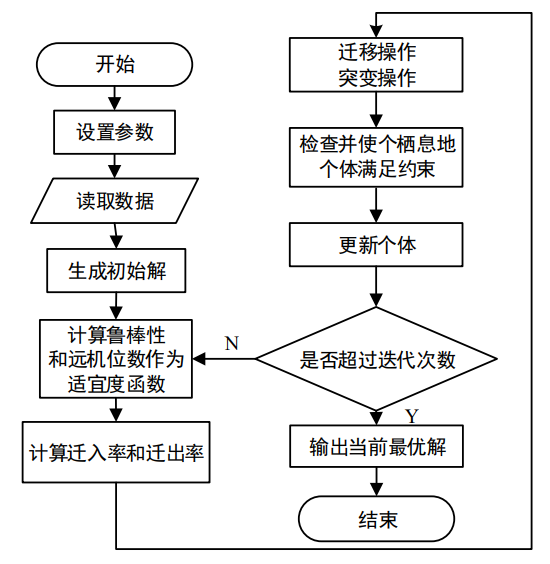
\includegraphics{BBO}
\caption{BBO算法流程图} \label{fig-BBO}
\end{figure}

\noindent(2)模型的求解过程 

该模型涉及到复杂的规划问题,目标函数为双目标多约束优化模型,而根据问题一的要求,两个目标函数的优先顺序为航班分配失败率最小$Z_1$,登机口使用比率最小$Z_2$。在进行求解的过程中,不断改变两个个目标函数的权重,从而得到一个总体程度最优的解。本模型中增加一个临时登机口,类别不受限制,数量不受限制,为分配失败的飞机提供临时登机口。

1、根据题目中的信息提示我们需要对 InputData.xlsx 进行数据预处理,对Pucks 附件中的数据提取出 20 日到达或 20 日出发的航班,其中包括 19 日到达20 日出发的航班信息,同时对 Gates 附件中登机口的字符进行量化标记便于后续处理。

2、确定不同飞机转场记录号(aircraft\_rn)的到达航班类型(arrive\_type)、出发航班类型(depart\_type)、飞机型号(aircraft\_jx)等信息;

\subsection{求解结果与分析}
\noindent(1)航班分配情况  \par
采用 BBO 算法对模型进行求解,得到航班分配成功数量为 498 个,航班分配成功比例为 82.18\%;被使用登机口数量为 65 个,被使用登机口比例为 94.2\%。根据航班分配登机口的结果,按宽、窄体机类型分别画出航班分配成功的数量和比例,如图 \ref{fig-航班成功分配数量},\ref{fig-航班成功分配比例} 所示。可以看出,宽体机的分配成功率达到 97.96\%,窄体机的分配成功率也达到 79.13\%。
\begin{figure}[h]

\begin{minipage}{0.45\textwidth}
\centering
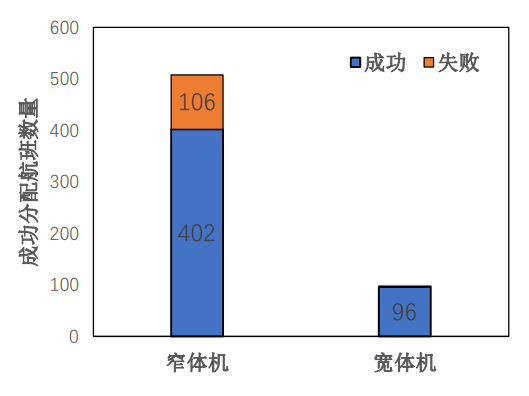
\includegraphics[scale=0.5]{航班成功分配数量}
\caption{航班成功分配数量} \label{fig-航班成功分配数量}
\end{minipage}
\begin{minipage}{0.45\textwidth}
\centering
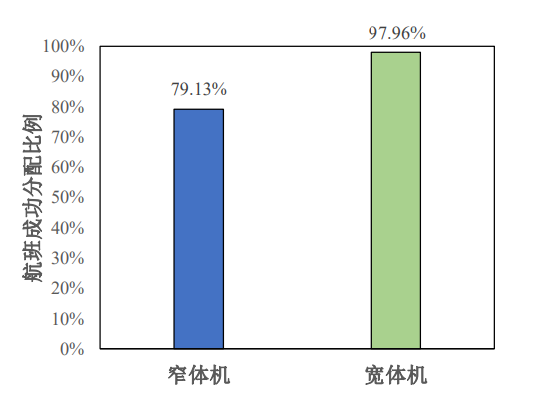
\includegraphics[scale=0.5]{航班成功分配比例}
\caption{航班成功分配比例} \label{fig-航班成功分配比例}
\end{minipage}

\end{figure}

\noindent (2) 登机口使用情况 

根据问题一的航班分配结果绘制甘特图,直观体现登机口的利用效果,如图\ref{fig-甘特图}所示。
\begin{landscape}
\begin{figure}
\centering
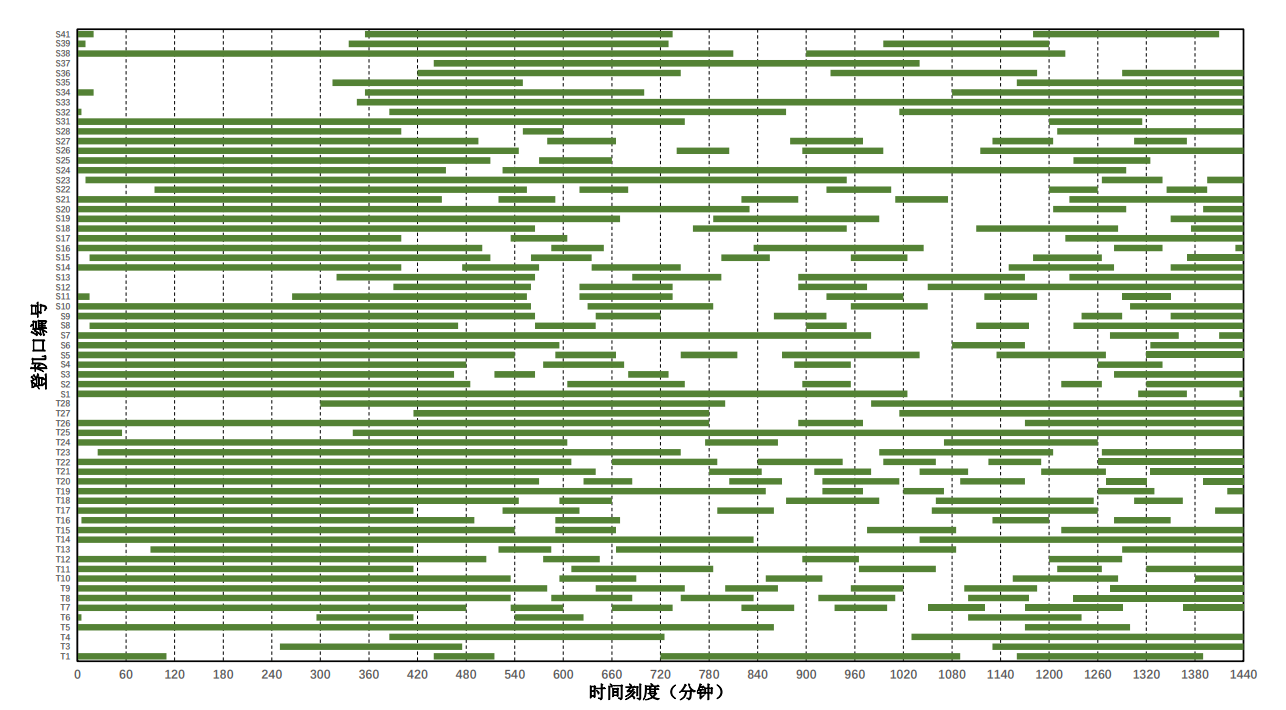
\includegraphics[width=25cm,height=15cm]{甘特图}
\caption{基于问题一航班分配结果的甘特图} \label{fig-甘特图}
\end{figure}
\end{landscape}


\section{问题二模型的建立与求解}
\subsection{问题的描述与分析}
考虑中转旅客最短流程时间的航班—登机口分配问题。本问题是在问题一的基础上加入旅客换乘因素:首先要求航班分配成功的数量最大,其次要求最小化中转旅客的总体最短流程时间,并且在此基础上最小化被使用登机口的数量。其中,中转旅客的总体最短流程时间只包括在不同登机口的转换时间,并不包括捷运时间和旅客的行走时间。
\subsection{模型的求解}     \par  XXXXXX 
\subsection{求解结果与分析} \par  XXXXXX

\section{问题三模型的建立与求解}
\subsection{问题的描述与分析}
考虑中转旅客最短流程时间的航班—登机口分配问题。本问题是在问题一的基础上加入旅客换乘因素:首先要求航班分配成功的数量最大,其次要求最小化中转旅客的总体最短流程时间,并且在此基础上最小化被使用登机口的数量。其中,中转旅客的总体最短流程时间只包括在不同登机口的转换时间,并不包括捷运时间和旅客的行走时间。
\subsection{模型的求解}     \par  XXXXXX 
\subsection{求解结果与分析} \par  XXXXXX

\section{模型的对比分析}

针对三个问题总共获得五个模型,分别是针对问题一的模型、针对问题二、三的未加入对临时机位的惩罚机制的模型、加入对临时机位的惩罚机制的模型。将五个模型的所有求解结果所对应的各类指标进行计算并整理成表格,如表 7-1 所示,结合该表格比
较模型之间的差异并分析产生原因:

(1)问题一、二和三模型纵向对比分析 \par
问题一的首要目标是尽可能的分配航班到合适的登机口,而在问题二和问题三未考虑对临时机位进行惩罚的模型中,需要进一步流程时间和乘客换乘因素,因此削弱了尽可能的分配航班到合适的登机口这一首要目标的权重,因此在以上三个模型中,第一个
模型的成功分配航班比率是最高的,达到 82.18\%;问题二中未考虑对临时机位进行惩罚的模型获得了所有模型中最小的总最短流程时间 50350 分钟;问题三中未考虑对临时机位进行惩罚的模型获得了所有模型中最低的总紧张度 454.33。

(2)问题二模型横向对比分析

(3)问题三模型横向对比分析

\begin{table}[htbp]
\centering
\caption{模型求解结果对应各类指标对比} 
\resizebox{\textwidth}{!}{
\begin{tabular}{*{9}{m{1.5cm}<{\centering}}}
\toprule[0.2em]
       &    & 成功分配航班比例  & 登机口使用数量 & 登机口平均使用率  & 正确换乘人数 & 总最短流程时间 (min) & 总换乘时间 & 总紧张度 \\ \hline
\multicolumn{2}{c}{问题一模型} &  82.18\%  &  65 & \textbf{61.25\%} & 1926 & 65725 & 67513  &591.11\\ \hline
\multirowcell{2}{问题\\二\\模型} & 未加入惩罚项 & 77.56\% & \textbf{64} & 58.45\% & 1554 & \textbf{50350} & \textbf{53838} & 474.65 \\ \cline{2-9}
  & 加入惩罚项 & 80.86\% & 67 & 59.51\% & \textbf{2052} & 69480 & 71549 & 630.70 \\ \hline      
\multirowcell{2}{问题\\三\\模型} & 未加入惩罚项 & 79.21\% & 66 & 57.96\% & 1588 & 53485 & 54094 & \textbf{454.33} \\ \cline{2-9}
  & 加入惩罚项 & \textbf{82.84}\% & 66 & 60.62\% & 2025 & 68255 & 69417 & 607.26 \\ 
\bottomrule[0.2em]
\end{tabular}}
\end{table}

\section{模型的总结与评价}
\subsection{模型的总结} \par
XXXXXX
\subsection{模型的评价} \par
XXXXX


\section{参考文献}
%参考文献
\bibliographystyle{gbt}
\bibliography{MathModel}

\newpage
%附录
\appendix
\section{程序代码}
%设置不同语言即可。
\begin{lstlisting}[language=Matlab] 
kk=2;[mdd,ndd]=size(dd);
while ~isempty(V)
[tmpd,j]=min(W(i,V));tmpj=V(j);
for k=2:ndd
[tmp1,jj]=min(dd(1,k)+W(dd(2,k),V));
tmp2=V(jj);tt(k-1,:)=[tmp1,tmp2,jj];
end
tmp=[tmpd,tmpj,j;tt];[tmp3,tmp4]=min(tmp(:,1));
if tmp3==tmpd, ss(1:2,kk)=[i;tmp(tmp4,2)];
else,tmp5=find(ss(:,tmp4)~=0);tmp6=length(tmp5);
if dd(2,tmp4)==ss(tmp6,tmp4)
ss(1:tmp6+1,kk)=[ss(tmp5,tmp4);tmp(tmp4,2)];
else, ss(1:3,kk)=[i;dd(2,tmp4);tmp(tmp4,2)];
end;end
dd=[dd,[tmp3;tmp(tmp4,2)]];V(tmp(tmp4,3))=[];
[mdd,ndd]=size(dd);kk=kk+1;
end; S=ss; D=dd(1,:);
 \end{lstlisting}

\end{document} 